\chapter{実験結果と考察}

\section{評価方法}
%入力希釈木の変形操作を用いた場合と用いなかった場合での希釈木のマッピング結果を比較して,
%入力希釈木の変形操作のFlushing操作を減少させる効果を評価する.
提案手法における希釈木の変形操作の評価を行うため,変形操作を行った希釈木と変形操作を行わなかった希釈木のそれぞれを入力として,
PMD上での液滴移動のない混合手順の生成を行った.
その後,それぞれの希釈木に対する混合手順において必要となったフラッシングの回数を比較することで,
希釈木の変形操作によるフラッシングの回数の削減率を求め,希釈木の変形操作の有効性を測った.

具体的な評価方法を述べる.
まず,高さ3,高さ4,高さ5のそれぞれの高さの希釈木を,500個ずつランダムに生成した.
その後,それぞれの高さごとの,すべての希釈木に関して,変形操作を行った希釈木と変形操作を行わなかった希釈木のそれぞれを入力とし,
PMD上での液滴移動のない混合手順の生成を行った.
これによって得られた混合手順の内,
変形操作を行った希釈木と変形操作を行わなかった希釈木の,どちらを入力として得られた混合手順も,
必要となるフラッシング回数が1以上だった場合のみ,希釈木の変形操作によるフラッシング回数の削減率を求めた.
そして,それぞれの高さごとにこの削減率の平均(平均削減率)を求め,希釈木の変形操作のフラッシング回数の削減における有効性を測った.

\section{実験結果と考察}
%実験結果を表で載せる.実験結果から分かることや考察を述べる. 
表~\ref{table:result}に実験結果を示した.
また,図~\ref{fig:graph}には3,4,5の各高さの希釈木における,変形操作によるフラッシングの回数の削減率をグラフで示した.

まずは,実験結果から分かることを述べる.
図~\ref{fig:graph}より,希釈木の高さが3,4,5と大きくなるにつれて,希釈木の変形操作によるフラッシングの回数の削減率は高くなっていることが分かる.
希釈木の高さが最も小さい3のときは,フラッシングの回数の平均削減率は-0.29$\%$と負の値をとっており,希釈木の変形操作によってフラッシングの回数が増加したことが分かる.

次に,以上で述べた実験結果に対する考察を述べる.
%希釈木の高さが3のときの希釈木の変形によるフラッシングの回数の平均削減率が負になっていることと,変形操作の対象になる希釈木の高さが大きくなるほど,フラッシングの回数の平均削減率が高まっていることから,
本実験結果より,
現在の希釈木の変形操作の手法で有効な変形を行うためには,高さの大きい希釈木を扱う必要があると考えた.
この理由は,2つ考えられる.

まず,1つ目の理由を述べる.
高さの大きい希釈木になるほど,その希釈木における深さの小さい位置にあるミキサーノードは多くの子孫ミキサーノードを持つため,割り当てられる予測混雑度の値は大きくなりやすい.
これにより,高さの大きい希釈木における,深さの小さい位置にあるミキサーノード間でも,割り当てられた予測混雑度の値の差は大きくなり,誤差での位置の入れ替えは少なくなる.
したがって,高さの大きい希釈木における,深さの小さい位置にあるミキサーノードに対するオーバーラップの起こしやすさの評価指標として,予測混雑度が上手くはたらき,フラッシングの回数の削減につながったのだと考えた.

次に,2つ目の理由を述べる.
表~\ref{table:result}から分かるように,希釈木の高さが大きいほど,希釈木内に含まれる2$\times$2ミキサーや2$\times$3ミキサーの平均個数も大きくなる.
これにより,希釈木の高さが大きいほど,それに対応した混合手順内で必要になるフラッシングの絶対数は増加する.
したがって,希釈木の高さが大きいほど,それに対応した混合手順内で必要になるフラッシングの回数の削減は容易になり,フラッシングの回数の平均削減率が高くなったのだと考えた.

\begin{table}[tbp]
\centering
\caption{実験結果}
\begin{tabular}{l|r|r|r} \Hline
\multicolumn{1}{l|}{希釈木の高さ}& \multicolumn{1}{l|}{2$\times$2ミキサー平均個数} &  \multicolumn{1}{l|}{2$\times$3ミキサー平均個数} & \multicolumn{1}{l}{フラッシングの平均削減率($\%$)} \\\hline\hline
3  & 3.26 & 4.16 & -0.29 \\\hline
4  & 7.17&9.06&2.92  \\\hline
5  & 13.37&17.67&5.18  \\\hline
\end{tabular}
\label{table:result}
\end{table}

\begin{figure}[tbp]
 \centering 
    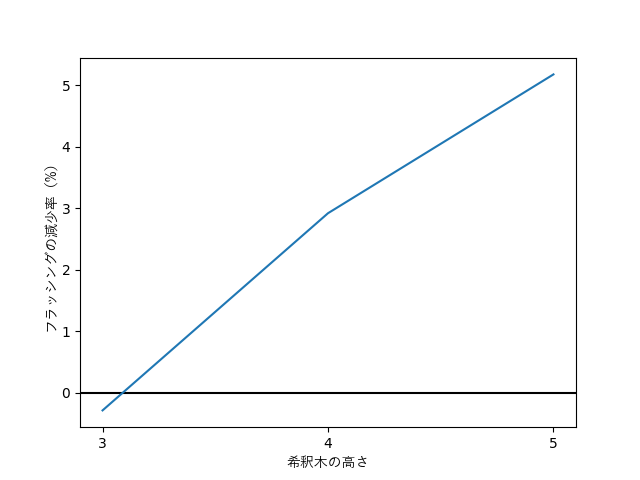
\includegraphics[scale=1.0]{img/decreasement.png}
 \caption{3,4,5のそれぞれの高さを持つ希釈木の,変形操作によるフラッシングの回数の平均削減率}\label{fig:graph}
\end{figure}
